\documentclass{article}
\usepackage{amsmath}
\usepackage{amssymb}
\usepackage[compact]{titlesec}
\usepackage{xcolor}
\usepackage{graphicx}
\usepackage{tikz}
\usetikzlibrary{calc,fadings,decorations.pathreplacing,shapes,shapes.multipart,arrows,shapes.misc,intersections,positioning}
\usepackage{wrapfig}
\usepackage{bm}
\usepackage{todonotes}

\graphicspath{{./}{./images/}}

\renewcommand{\vec}[1]{\boldsymbol{\mathbf{#1}}}
\newcommand{\tr}[0]{\text{tr}}
\newcommand{\norm}[1]{\left\lVert#1\right\rVert}

\tikzset{
    partial ellipse/.style args={#1:#2:#3}{
        insert path={+ (#1:#3) arc (#1:#2:#3)}
    }
}

\textwidth = 6.5 in
\textheight = 9 in
\oddsidemargin = 0.0 in
\evensidemargin = 0.0 in
\topmargin = 0.0 in
\headheight = 0.0 in
\headsep = 0.0 in
\parskip = 0.2in
\parindent = 0.0in

% configure hyperref to remove ugly boxes from links
\definecolor{darkblue}{rgb}{0.1,0.2,0.6} \definecolor{darkred}{rgb}{0.8,0.1,0.2}
\usepackage[colorlinks,citecolor=darkblue,linkcolor=darkred,urlcolor=darkblue]{hyperref}

\title{Boundary Conformal Field Theory}
\author{Tianci Zhou}

\begin{document}
\maketitle
\large


\section{Conformal Interface of Free Boson}
% flatex input: [boson_interface.tex]
\label{sec:var-boson}
[Section 2.1-2.2 of \cite{bachas_permeable_2002}.]

Let's consider the conformal interface connecting two possibly different free boson CFTs. Suppose the interface is located at $x = 0$ that glues the two theories in such a way that 
\begin{equation}
\begin{bmatrix}
\partial_t \phi\\
\partial_x \phi\\ 
\end{bmatrix}_{x = 0^-} 
 = M \begin{bmatrix}
\partial_t \phi\\
\partial_x \phi\\ 
\end{bmatrix}_{x = 0^+} 
\end{equation}
One may write the field on the left/right as $\phi^1$($\phi^2$), and then the gluing condition is
\begin{equation}
\partial_{\mu} \phi^1 = M_{\mu\nu} \partial_{\nu} \phi^2 
\end{equation}
The interface is now penetrable, and condition \eqref{eq:stress-cond} is weakened that only requires continuity of the momentum across the interface. From the explicit expression
\begin{equation}
T^{xt} = - g \partial_x \phi \partial_t \phi  = -g(\partial_{\mu} \phi \sigma^x_{\mu\nu}  \partial_{\nu} \phi ) 
\end{equation}
we have the relation
\begin{equation}
\partial_{\mu} \phi^2 \sigma^x_{\mu\nu}  \partial^2_{\nu} \phi -  \partial_{\mu} \phi^1 \sigma^x_{\mu\nu}  \partial^1_{\nu} \phi = 
\partial_{\mu} \phi^2 [\sigma^x_{\mu\nu} - M^T  \sigma^x M)_{\mu\nu} ]  \partial_{\nu} \phi^2 = 0
\end{equation}
For generic field configuration $\phi^2$, the condition is satisfied only when
\begin{equation}
\sigma^x = M^T \sigma^x M 
\end{equation}
By diagonalizing $\sigma^x$ and doing corresponding orthogonal transformation on $M$, 
\begin{equation}
\sigma^z = ( OMO^T  )^T \sigma^z ( OMO^T )  \quad 
O = \frac{1}{\sqrt{2}} 
\begin{bmatrix}
1 & 1 \\
1 & -1 \\                       
\end{bmatrix}
\end{equation}
we realize $O M O^T$ is in the Lorentz group $O( 1, 1 )$, whose 4 disconnected components that are determined by the sign of determinants and the $00$ element. A natural boost parameterization are 
\begin{equation} 
\Lambda = O M O^T = \pm 
\begin{bmatrix}
\cosh \beta & \sinh \beta \\
\sinh \beta & \cosh \beta \\  
\end{bmatrix}
\quad \pm 
\begin{bmatrix}
\cosh \beta & -\sinh \beta \\
\sinh \beta & -\cosh \beta \\  
\end{bmatrix}
\end{equation}
Reverting back to $M$, we have $\lambda = e^{-\beta}$
\begin{equation}
M_1 = \pm 
\begin{bmatrix}
\lambda^{-1} & 0 \\
0 & \lambda \\
\end{bmatrix}
\quad 
M_2 = \pm 
\begin{bmatrix}
0 & \lambda\\
\lambda^{-1} & 0 \\
\end{bmatrix}
\end{equation}
The $\pm$ branches in each $M$ can be combined if we set $\lambda = \text{tan} \theta$ for $\theta \in [- \frac{\pi}{2}, \frac{\pi}{2} ] $.

The physical significance of $\theta$ can be seen in the following scattering picture. The solutions of equation of motion are the left and right moving waves. The derivative $\partial_{-} = \partial_t - \partial_x$ removes the left moving component($x+t$) and hence can generate right moving fields $\partial_{-} \phi$. The process of right moving $\phi^1$ combined with left moving $\phi^2$ to generate a left moving $\phi^1$ and right moving $\phi^2$
\begin{equation}
\partial_{-} \phi^1 + \partial_{+} \phi^2 \rightarrow \partial_{+} \phi^1 + \partial_{-} \phi^2
\end{equation}
can be described by the scattering matrix
\begin{equation}
\begin{bmatrix}
\partial_{+} \phi^1 \\
\partial_{-} \phi^2 \\
\end{bmatrix}
 = S
\begin{bmatrix}
\partial_{-} \phi^1 \\
\partial_{+} \phi^2 \\
\end{bmatrix}
\end{equation}
After some linear algebra, we find that $2\theta$ is the angle that parameterize the scattering matrix\footnote{I adopt several different conventions from \cite{bachas_permeable_2002}. 1. I put $\partial_t$ as the first entry of the vector. 2. The matrices $M(\lambda)$ is actually $M(\lambda^{-1} )$ in \cite{bachas_permeable_2002}. These two cancel out and the resulting gluing conditions are the same. 3. I take $\partial_{-} \phi^1, \partial_{+} \phi^2$ as incoming wave, so that the $S$ matrix maps it to the outgoing waves, while \cite{bachas_permeable_2002} use the opposite: they obtain $S^{-1}$. Incidentally, $S = S^{-1}$. 4. I take $\partial_{-} = \partial_t - \partial_x $, while \cite{bachas_permeable_2002} seems to take $\partial_{-} = \partial_x - \partial_t$. Interchanging $x$ and $t$ amounts to change $\lambda$ to $\lambda^{-1}$, or $\theta$ to $\frac{\pi}{2}- \theta$, which indeed converts $S$ here to the $S$ in \cite{bachas_permeable_2002}. }
\begin{equation}
\label{eq:S1-S2}
S_1 =
\begin{bmatrix}
\cos 2 \theta & \sin 2 \theta \\
\sin 2 \theta & - \cos 2 \theta     
\end{bmatrix}
\qquad
S_2 = 
\begin{bmatrix}
-\cos 2 \theta & \sin 2 \theta \\
-\sin 2 \theta & - \cos 2 \theta   
\end{bmatrix}
\end{equation}

\subsection{Example: Free Boson with Different Compactification Radii}

[Section 2.2 of \cite{bachas_permeable_2002}.]

Suppose $\phi^1$ and $\phi^2$ are compact Bosons with compactification radii $2\pi R_1$ and $2\pi R_2$. We can rescale them to a single field 
\begin{equation}
\phi = \left\lbrace
       \begin{aligned}
         R_1^{-1} \phi^2  & \quad  x < 0 \\
         R_2^{-1} \phi^2  & \quad x > 0  \\
       \end{aligned} \right. 
\end{equation}
such that $\phi$ is a compact boson on the whole plane with radius $2\pi$, whose action(in Euclidean time) reads
\begin{equation}
S = \frac{g}{2} R_1^2 \int_{x \le 0 } \left(  \nabla \phi \right)^2 d\tau dt  + \frac{g}{2} R_2^2 \int_{x > 0 } \left(  \nabla \phi  \right)^2 d\tau dt 
\end{equation}
Both the bulk action as well as the interface should be invariant under the conformal transformation. We do such a conformal transformation, which induces a change on the field $\phi \rightarrow \delta \phi $, and since the bulk is invariant, we only need to check the boundary term
\begin{equation}
S = \frac{g}{2} \int_{x = 0 } ( R_1^2 \partial_x \phi\big|_{x = 0^{-}}   - R_2 ^2 \partial_x \phi \big|_{x = 0^{+}} ) \delta \phi  d\tau = 0
\end{equation}
The boundary condition
\begin{equation}
R_1^2 \partial_x \phi\big|_{x = 0^{-}}  = R_2 ^2 \partial_x \phi \big|_{x = 0^{+}}
\end{equation}
which makes any variation vanish must be conformal invariant. In terms of the $\phi^1$, $\phi^2$ fields
\begin{equation}
\partial_x \phi^1 = \frac{R_2}{R_1} \partial_x \phi^2 
\end{equation}
According to our previous analysis, it corresponds to $M_1$ with $\lambda = \frac{R_2}{R_1} = \tan \theta$, namely
\begin{equation}
\label{eq:cpt_boson_bd}
\partial_t ( \cos \theta \phi^1  - \sin \theta \phi^2 ) = 0 \qquad \partial_x ( \sin \theta \phi^1  - \cos \theta \phi^2 ) = 0
\end{equation}


%%% Local Variables:
%%% TeX-master: "bCFT_notes"
%%% TeX-PDF-mode: t
%%% End:

% flatex input end: [boson_interface.tex]

% configure hyperref to remove ugly boxes from links

\subsection{Folding Trick and Boundary State}
% flatex input: [folding.tex]


[Section 2.3-2.4 of \cite{bachas_permeable_2002}]

We can fold the field $\phi^2$ to the left half plane on top of $\phi^1$, then the boundary at $x = 0$ is impenetrable for the tensor theory and therefore is a boundary state of Boson. 

The folding takes $x$ to $-x$ in $\phi^2$, so its $x$ derivative in the boundary condition \eqref{eq:cpt_boson_bd} will change sign and becomes\footnote{Change $\theta$ to $\frac{\pi}{2} - \theta$ to compare relevant result with in \cite{bachas_permeable_2002}. I believe the \cite{bachas_permeable_2002} made a mistake here. Nevertheless the Casimir energy is insensitive to this change.},
\begin{equation}
\partial_t ( \cos \theta \phi^1  - \sin \theta \phi^2 ) = 0 \qquad \partial_x ( \sin \theta \phi^1  + \cos \theta \phi^2 ) = 0
\end{equation}
It looks like the rotated field within $\partial_t$ takes Dirichlet boundary condition and the other orthogonal field within $\partial_x $ takes Neumann boundary condition, so we have\footnote{We will deal with the winding sector in Sec.~\ref{sec:winding}}
\begin{equation}
\label{eq:rot-D-N}
\begin{aligned}
\cos  \theta a^1_n - \sin \theta a^2_n  &= + \left( \cos  \theta \bar{a}^1_{-n} - \sin \theta \bar{a}^2_{-n} \right)\\
\sin  \theta a^1_n + \cos \theta a^2_n  &= - \left( \sin  \theta \bar{a}^1_{-n} + \cos \theta \bar{a}^2_{-n} \right) 
\end{aligned}
\end{equation}
The left and right sides can be regarded as two new sets of $a^1$ and $a^2$ whose commutation relation is preserved by the orthogonal rotation. Consequently, the boundary state is
\begin{equation}
\label{eq:bd_state}
\begin{aligned}
| B \rangle &= \exp\Big\{ \sum_{n > 0 } \frac{1}{n} (\cos  \theta a^1_{-n} - \sin \theta a ^2_{-n} )(\cos  \theta \bar{a}^1_{-n} - \sin \theta \bar{a}^2_{-n} ) \\
& \,\,  \qquad \qquad -\frac{1}{n} (\sin  \theta a^1_{-n} + \cos \theta a ^2_{-n} )(\sin  \theta \bar{a}^1_{-n} + \cos \theta \bar{a}^2_{-n} )
\Big\} | 0 \rangle \\
& = \exp\Big\{ \sum_{n > 0 } \frac{1}{n} \left( \cos 2\theta a^1_{-n} \bar{a}^1_{-n}  - \cos 2\theta a ^2_{-n} \bar{a}^2_{-n}   
- \sin 2 \theta a ^2_{-n}\bar{a}^1_{-n}  - \sin 2 \theta a ^1_{-n}\bar{a}^2_{-n}  \right ) \Big\}| 0 \rangle \\
& =  \exp\Big\{ \sum_{n > 0 } \frac{1}{n}
\begin{bmatrix}
a_{-n}^1\\
a_{-n}^2\\                              
\end{bmatrix}
S_1
\begin{bmatrix}
\bar{a}_{-n}^1  \bar{a}_{-n}^2
\end{bmatrix} \Big\}
\end{aligned}
\end{equation}

%%% Local Variables:
%%% TeX-master: "bCFT_notes"
%%% TeX-PDF-mode: t
%%% End:
% flatex input end: [folding.tex]

% configure hyperref to remove ugly boxes from links


\section{Compact Boson Winding Modes}
\label{sec:winding}
% flatex input: [D_and_N.tex]

\subsection{Dirichlet and Neumann Boundary Conditions}

[Section 2 of \cite{bachas_fusion_2008}, Section 6.3.5 of \cite{di_francesco_conformal_1997}]

The winding modes of compact boson determines the conformal dimensions of the primary fields. It therefore restrict possible bcc operators on the boundary. In this section we work the simple Dirichlet and Neumann conditions for the winding modes.

{\bf Mode Expansion:} 
Suppose the boson is compactified as $\phi \rightarrow \phi + 2\pi R$, then mode expansion in Eq.~\ref{eq:boson-mode-exp} will have a different zero mode\footnote{The sign of the $x$ term is different from Eq. (6.91) in \cite{di_francesco_conformal_1997}, but calculation later shows that the $-$ sign is correct to give the $(\frac{n}{4\pi gR} + \frac{1}{2} \frac{m}{R})$ combination for $z$. }  
\begin{equation}
\begin{aligned}
\phi( x, t ) &= \phi_0 - \frac{2\pi m R}{L}x + \frac{\pi_0}{gL} t  + \text{oscillator part}  \\
&= \phi_0 - \frac{2\pi m R}{L}x + \frac{n}{gLR} t  + \text{oscillator part}  \\
\end{aligned}
\end{equation}
where the conjugate momentum $\pi_0$ takes discrete eigenvalues $\frac{n}{R}$. A particle living on unit circle $[0, 2\pi]$ have integer($m \hbar$) angular momentum(conjugate momentum), and so momentum of Boson living on $[0, 2\pi R]$ will have $\frac{n}{R}$ as its eigenvalues. 

The left and right mode decomposition is again done by complex variables
\begin{equation}
z = \exp( 2 \pi i \frac{t - x}{L}) \qquad \bar{z} = \exp( 2 \pi i \frac{t + x}{L})
\end{equation}
which leads to
\begin{equation}
\label{eq:boson-mode-exp}
\begin{aligned}
\phi( z, \bar{z}) = &\phi_0 -i \left( \frac{n}{4\pi g  R} + \frac{m R }{2} \right)  \ln z + \frac{i}{\sqrt{4\pi g}} \sum_{n\ne 0 } \frac{a_n}{n} z^{-n } \\
&-i \left( \frac{n}{4\pi g R} - \frac{m R }{2} \right)  \ln \bar{z} + \frac{i}{\sqrt{4\pi g}} \sum_{n\ne 0 } \frac{\bar{a}_n}{n} \bar{z}^{-n } 
\end{aligned}
\end{equation}
From the holomorphic derivative 
\begin{equation}
i \partial_z \phi =  \sum_n \frac{1}{\sqrt{4\pi g}} a_n z^{-n-1}  \qquad a_0 = \sqrt{ 4 \pi g } \left( \frac{n}{4\pi g R} + \frac{m R }{2} \right)
\end{equation}
we make up the zero mode term in $L_0$ is absent for free boson, 
\begin{equation}
L_0 = \sum_{n> 0 } a_{-n} a_n + \frac{1}{2} a_0^2 =   2\pi g \left( \frac{n}{4\pi g R} + \frac{m R }{2} \right)^2 + \sum_{n> 0 } a_{-n} a_n
\end{equation}
The ground state now has dimension $h = 2\pi g \left( \frac{n}{4\pi g R} + \frac{m R }{2} \right)^2$. 

{\bf Dirichlet and Neumann}:

Now that we have a legitimate $a_0$ that behaves similar with other oscillator modes, we can then impose the same Dirichlet condition in Eq.~\ref{eq:D-mode-cond}, on the unit circle, the logarithmic term gives 
\begin{equation}
 -i \frac{1}{\sqrt{ 4\pi g}}  ( a_0 \ln z  + \bar{a}_0 \ln \bar{z} )\Big|_{\text{unit circle }} = 0 \quad \implies \quad a_0 - \bar{a}_0 = 0  \quad \implies \quad m = 0
\end{equation}
The boundary states satisfying this boundary condition can be a linear superposition of the zero winding states. Since it's Dirichlet, it is an eigenstate of $\hat{\phi}_0$\footnote{We have quantized the theory such that $[\phi_0, \frac{n}{R}] = i $. },
\begin{equation}
|{\rm D} \rangle  = g_{\,\!_\text{D}}  \prod_{n > 0 } \exp(\frac{1}{k} a_k^{\dagger} \bar{a}_{-k}^{\dagger} )| \phi_0 \rangle \quad | \phi_0 \rangle = \sum_{n \in \mathbb{Z}} e^{-i \frac{n}{R}\phi_0 } | n, m = 0 \rangle  
\end{equation}
With this one can show
\begin{equation}
\phi( x, t = 0 ) | {\rm D} \rangle = \phi_0 | {\rm D} \rangle
\end{equation}

Similarly, the Neumann boundary condition now has the $n = 0$ term in Eq.~\ref{eq:N-mode-cond}
\begin{equation}
 a_0 + \bar{a}_0 = 0  \quad \implies \quad n = 0 
\end{equation}
the resulting boundary state is a linear superposition over the winding sector
\begin{equation}
| {\rm N} \rangle = g_{\,\!_\text{N}} \prod_{n > 0 } \exp(\frac{1}{k} a_k^{\dagger} \bar{a}_{-k}^{\dagger} )| \bar{\phi}_0 \rangle \quad | \bar{\phi}_0 \rangle = \sum_{n \in \mathbb{Z}} e^{i m \bar{\phi}_0 } | n = 0, m \rangle 
\end{equation}
In fact, Neumann becomes Dirichlet in the dual field, so $\bar{\phi}_0$ is related to the boundary value of the dual field. 

One can check that this indeed satisfies the Neumann boundary condition
\begin{equation}
\partial_t \phi( x, t = 0 ) | {\rm N } \rangle = 0
\end{equation}

%%% Local Variables:
%%% TeX-master: "bCFT_notes"
%%% TeX-PDF-mode: t
%%% End:
% flatex input end: [D_and_N.tex]

% configure hyperref to remove ugly boxes from links
\subsection{Gluing Condition for Winding Modes}
% flatex input: [glue_zero.tex]
[Appendix A of Oshikawa\cite{oshikawa_boundary_2010}]

In Sec.~\ref{sec:var-boson}, we use variational approach to find conformal invariant boundary conditions, but the resulting equation \eqref{eq:cpt_boson_bd} do not provide information about the winding sector. The variational method fails because winding is a global properties of the Boson configuration, meaning insensitive to the local perturbation. 

Here we present a general treatment about the winding modes. From the discussion of the Dirichlet and Neumann boundary condition in previous subsection, it seems that the constraints on the oscillator modes can be naturally extended to the zero mode for $n = 0$. We can show that this is in compliance with the conformal invariance. 

Suppose in the junction we have a boundary condition that result in the following scattering relation
\begin{equation}
\begin{bmatrix}
\partial_{+} \phi^1 \\
\partial_{-} \phi^2 \\
\end{bmatrix}
 = S
\begin{bmatrix}
\partial_{-} \phi^1 \\
\partial_{+} \phi^2 \\
\end{bmatrix}
\end{equation}
the conformal invariance constraint gives two solutions $S_1$ and $S_2$ in Eq.~\eqref{eq:S1-S2}. Imagining that we fold $\phi^2$ on top of $\phi^1$, the $x$ derivative on $\phi^2$ then changes sign, we therefore have
\begin{equation}
\begin{bmatrix}
\partial_{+} \phi^1 \\
\partial_{+} \phi^2 \\
\end{bmatrix}
 = S
\begin{bmatrix}
\partial_{-} \phi^1 \\
\partial_{-} \phi^2 \\
\end{bmatrix}
\end{equation}
It it convenient to work in the holomorphic mode expansion \eqref{eq:boson-mode-exp} for the left and right separation. Specifically
\begin{equation}
\partial_{+} = \frac{4\pi i }{L} \bar{z} \partial_{\bar{z}} \qquad \partial_{-} = \frac{4\pi i }{L} z\partial_{z}
\end{equation}
and
\begin{equation}
\sum_{n \in \mathbb{Z}}  
\begin{bmatrix}
\bar{a}^1_{n} \bar{z}^{\scalebox{0.5}[0.8]{\( - \)}n}\\ 
\bar{a}^2_{n} \bar{z}^{\scalebox{0.5}[0.8]{\( - \)}n} 
\end{bmatrix}
 = S
\sum_{n \in \mathbb{Z}}
\begin{bmatrix}
a^1_n z^{\scalebox{0.5}[0.8]{\( - \)}n} \\
a^2_n z^{\scalebox{0.5}[0.8]{\( - \)}n} \\
\end{bmatrix}
\end{equation}
We impose boundary condition at $t = 0$\footnote{In Sec.~\ref{subsec:free-boson}, we interchange $x$ and $t$, and impose boundary condition at $x = 0$. For whatever convention, the boundary is on the unit circle $|z| = 1$. }, so $z$  is on the unit circle and $\bar{z} = \frac{1}{z}$. By comparing the modes(Fourier series on circle), we have
\begin{equation}
\label{eq:mode-eq}
a_n^i - (S^{\scalebox{0.5}[0.8]{\( - \)}1})_{ij} \bar{a}_{\scalebox{0.6}[0.6]{\( - \)}n}^j = 0
\end{equation}
This is clearly a generalization of the Dirichlet and Neumann boundary conditions, where the orthogonal matrix $S$ is replaced by $\pm \mathbb{I}$. In fact, the rotation does not change the quadratic relation
\begin{equation}
\sum_i a^i_n a^i_m =  \sum_i \bar{a}_{\scalebox{0.6}[0.6]{\( - \)}n}^i \bar{a}_{\scalebox{0.6}[0.6]{\( - \)}m}^i
\end{equation}
Hence for the quadratics in the Virasolo generators
\begin{equation}
\begin{aligned}
L_n &= \frac{1}{2} \sum_i  \sum_{m > -1 } (a^i_{n-m} a^i_m  + a^i_{-m} a^i_{n+m } ) - \frac{1}{2} a^i_0 a^i_n 
\end{aligned}
\end{equation}
the cancellation works the same way,
\begin{equation}
\begin{aligned}
L_n - \bar{L}_{-n} &= \frac{1}{2} \sum_i \sum_{m > -1} ( a^i_{n-m} a^i_m + a^i_{-m} a^i_{n+m} - \bar{a}^i_{-n-m} \bar{a}^i_{-m} - \bar{a}^i_{m} \bar{a}^i_{-n+m }  )  - \frac{1}{2}( a_0^i a_n^i - \bar{a}_0^i \bar{a}^i _{-n})\\
& = \frac{1}{2} \sum_i \sum_{m > -1} ( a^i_{n-m} a^i_m  - \bar{a}^i_{-n+m}\bar{a}^i_{-m})+ (a^i_{-m} a^i_{n+m} - \bar{a}^i_{m} \bar{a}^i_{-n -m }  )\\
& = 0 
\end{aligned}
\end{equation}
We now specialize to the two cases $S = S_1$ and $S_2$. 

{\bf Boson $\lambda$ Junction: $S = S_1$}

We need to solve the $n = 0$ of \eqref{eq:mode-eq} for $S^{-1} = S_1^{-1} = S_1$\footnote{Recall that the solution of Eq.~\eqref{eq:mode-eq} for the nonzero mode is $\exp(\frac{1}{n} a_{-n}^{i} S^{-1}_{ij} a_{-n}^j |0\rangle)$. In Eq.~\eqref{eq:R-bs} we do have $R = S_1$. } and
\begin{equation}
a^i_0 = \sqrt{4\pi g}  \frac{1}{4\pi} (2\pi m_i R_i + \frac{1}{g} \frac{n_i}{R_i})
\end{equation}
For notational simplicity, we introduce the compactification lattice and its dual\cite{oshikawa_boundary_2010}
\begin{equation}
\label{eq:lattice}
\vec{M} = (m_1 2 \pi R_1, m_2 2\pi  R_2)^\top, \quad  \vec{M}^* = (\frac{n_1}{R_1}, \frac{n_2}{R_2})^\top
\end{equation}
the constraint then becomes 
\begin{equation}
  a_0^i - S^{-1} _{ij} \bar{a}_{0}^j = 0 \quad \implies \quad ( \vec{M} + \frac{1}{g}\vec{M}^* ) = S_1 ( -\vec{M} + \frac{1}{g}\vec{M}^* )
\end{equation}
which is basically the two dimensional case of the multi-component Boson constraints in Eq.~(86) of \cite{oshikawa_boundary_2010}. 

Given the $S_1$ matrix in Eq.~\eqref{eq:S1-S2}, we have
\begin{equation}
1 + S_1 = 2  
\begin{bmatrix}
\cos^2 \theta & \sin \theta \cos\theta \\
\sin \theta \cos \theta  & \sin^2 \theta \\
\end{bmatrix}
\quad 
1 - S_1 = 2
\begin{bmatrix}
\sin^2 \theta & -\sin \theta \cos\theta \\
-\sin \theta \cos \theta  & \cos^2 \theta \\
\end{bmatrix}
\end{equation}
both have determinant zero. So the solution of the two lattice vectors in 
\begin{equation}
( 1 + S_1) \vec{M} = -( 1 - S_1 ) \frac{1}{g} \vec{M}^*
\end{equation}
must be the null vectors of the corresponding matrices, i.e. 
\begin{equation}
\vec{M} = ( \cos \theta, -\sin \theta )^\top \qquad \vec{M}^{*} = ( \sin \theta, \cos \theta )^\top 
\end{equation}
In terms of the winding numbers
\begin{equation}
  \tan \theta =  \frac{n_1 R_2}{n_2 R_1 } = -\frac{m_2 R_2}{ m_1 R_1}
\end{equation}
One can take a pair of coprime integers $k_1$ and $k_2$($k_1>0$), such that $-\frac{m_1}{m_2} = \frac{k_1}{k_2}$. That determines all the possible winding numbers of the basis\footnote{\cite{bachas_fusion_2008} takes $-S_1$ as the S matrix, so they have $\vec{M} = ( \cos \theta, \sin \theta)^\top $ and $\tan \theta = -\frac{n_1 R_2}{n_2 R_1 } = \frac{m_2 R_2}{ m_1 R_1} = \frac{k_2 R_2}{k_1 R_1}$ for $\frac{m_1}{m_2} = \frac{k_1}{k_2}$. And this is consistent with their parameterization  $ \left\lbrace
  \begin{aligned}
    m_1 = k_1 M  & \quad n_1 = k_2 N  \\
    m_2 = k_2 M &  \quad n_2 = -k_1 N \\
  \end{aligned} \right. $ }. The linear superposition is beyond conformal invariance, which should be determined by Cardy's consistency condition. 

This set of boundary conditions can be viewed as Dirichlet and Neumann on the rotated basis, hence a reasonable conjecture is also the Fourier sum of the basis(constrained by $S_1$)
\begin{equation}
g_{\,\!_{S_1}} \sum_{S_1} e^{i n_1 \phi_0 - i m_1 \bar{\phi}_0 } | n_1, m_1  \rangle | n_2, m_2  \rangle 
\end{equation}

{\bf The T-dual Boundary State $S = S_2$}

Now we take $S = S_2$, the zero mode condition becomes
\begin{equation}
( \vec{M} + \frac{1}{g}\vec{M}^* ) =  S_2^{-1}  ( -\vec{M} + \frac{1}{g}\vec{M}^* )
\end{equation}
the solution is
\begin{equation}
\vec{M} =  \frac{1}{g} \frac{1 - S_2}{1 + S_2} \vec{M}^{*} = \frac{1}{g}  \frac{1}{ 1 - \cos 2\theta}
\begin{bmatrix}
  0 & - \sin 2 \theta \\
\sin 2\theta & 0 \\
\end{bmatrix} \vec{M}^*
 = \frac{\cot \theta}{g} \begin{bmatrix}
  0 & - 1 \\
1 & 0 \\
\end{bmatrix}\vec{M}^*
\end{equation}
Using the basis vectors in Eq.~\ref{eq:lattice}, we have
\begin{equation}
\begin{bmatrix}
m_1\\
m_2\\
\end{bmatrix}
 = \frac{2 \cot \theta}{ 4\pi g  R_1 R_2 }
\begin{bmatrix}
-n_2 \\
n_1 
\end{bmatrix}
\end{equation}
Taking the same coprime interger $\frac{m_2}{n_1} = \frac{k_2}{k_1}$, we have the angle\footnote{It takes some effort to match the results with \cite{bachas_fusion_2008}. We both use $\frac{k_2}{k_1}$ the same way, so the parameterization is the same. They use $-S_2$ as oppose to $S_2$ to be the S matrix, so $\vec{M} = \frac{1}{g} \frac{1 + S_2}{1 - S_2} = \frac{\tan \theta}{g}\begin{bmatrix}
  0 & - 1 \\
1 & 0 \\
\end{bmatrix} \vec{M}^*$, their $\tan \theta$ is my $\cot \theta = \frac{k_2}{2k_1 } 4\pi g R_1 R_2$. They use $R \rightarrow \frac{1}{2R}$ as T-duality transformation. If they were to use $R \rightarrow \frac{1}{2R}$(this point corresponds to $g = \frac{1}{4\pi}$), then their $\tan \theta = \frac{k_2}{2 k_1} R_1 R_2$ which will be the same as our $\cot \theta$. So we agree.},
\begin{equation}
  \tan \theta = \frac{2 k_1}{k_2} \frac{1}{4 \pi g R_1 R_2}
\end{equation}
This state can be obtained by taking T duality for one of the bosons, hence it is a Dirichlet/Neumann boundary conditions for these two Bosons. It is then reasonable to use Fourier sum as the physical boundary state
\begin{equation}
g_{_{\,\!_{S_2}}}\sum_{S_2} e^{i n_1 \phi_0 - i m_1 \bar{\phi}_0 } | n_1, m_1  \rangle | n_2, m_2  \rangle 
\end{equation}

{\bf The $g$ Factor}: 

The $g$ factor can only be determined by Cardy condition, which means that the occurrence $n^h_{ab}$ for each irreducible representation
\begin{equation}
Z_{ab} = \langle a | e^{- \beta  H }  | b \rangle  = \sum_{h} n_{ab}^h \chi_h 
\end{equation}
is an non-negative integer. 

Since the character for the compact boson theory is known, we can just compute the amplitude, say $Z_{\lambda_1, \lambda_2}$ adjust the coefficient such the occurrence is an integer. \cite{bachas_fusion_2008} contains a calculation for Dirichlet case. I will not repeat it here. 

%%% Local Variables:
%%% TeX-master: "bCFT_notes"
%%% TeX-PDF-mode: t
%%% End:
% flatex input end: [glue_zero.tex]

% configure hyperref to remove ugly boxes from links
\subsection{Winding Modes Contribution to Partition Function}
% flatex input: [Z-winding.tex]

In this section, we address the concern about how the winding mode will affect the partition function.
\begin{figure}[h]
\centering
\begin{tikzpicture}[scale = 1]
\draw (0,0)--(2,0);
\draw (0,1.5)--++(2,0);
\node () at (1,-0.5) {$\lambda_1$};
\node () at (1,2) {$\lambda_2$};
\draw[-stealth] (1,0.5)--++(0,0.5);
\end{tikzpicture}
\caption{Partition function between two boundary states $\lambda_1$ and $\lambda_2$}
\label{fig:part-lambda1-lambda2}
\end{figure}

Let the cylinder to have width $\beta$ and the length of in time direction is $\pi$(after folding), we have
\begin{equation}
Z = \langle \lambda_2 | e^{-\pi H} | \lambda_1 \rangle   \qquad H = \frac{4\pi}{ \beta} L_0 
\end{equation}
For the winding mode part, we just replace $L_0$ to be $a_0$. When the two boundary states are identical, the result will be a theta-function
\begin{equation}
Z_0 = \sum_{S_1 } g_{\,\!_{\lambda_1} }g_{\,\!_{\lambda_2} } \exp\Big\{- \frac{4\pi}{\beta} 2 \pi g ( \frac{n_1}{ 4 \pi R_1 g} + \frac{m_1 R_1 }{ 2} )^2 \Big\}
\end{equation}
In the $\beta \rightarrow \infty$ limit, it will be proportional to $\beta$ by Poisson's resummation formula\footnote{One can also approximate the sum by integral in this limit: it will be a two dimensional Gaussian integral and the result is proportional to $\beta$}. So the winding mode part will at most contribute a $\ln \beta$ term in the free energy, which can be neglected in our leading $\beta$ scaling analysis. 

The conclusion still holds for different $\lambda$ boundary states, in which case the only change is the possible values of $n_1$ and $m_1$(the lattice). The overlap $\langle \lambda_1 | \lambda_2 \rangle $ will not be zero even if the two sets of coprime integers are different for the two boundary states: they can meet in their least common divisor. 


%%% Local Variables:
%%% TeX-master: "bCFT_notes"
%%% TeX-PDF-mode: t
%%% End:
% flatex input end: [Z-winding.tex]

% configure hyperref to remove ugly boxes from links

\section{Loschmidt Echo of Connecting Free Bosons}
\subsection{Corrections to Casimir Energy}
% flatex input: [free_boson_echo.tex]

To test our boundary state formalism, we consider the Loschmidt echo of connecting two (non-chiral) non-compact Bosons on the two half planes. 
% flatex input: [fig_H_tau.tex]


\begin{figure}[h]
\centering
\begin{tikzpicture}[scale = 2]
\draw (0,0) --(0.9,0);
\draw (2.1,0)--++(.9,0);
\node[below] () at (1,-0.15) {$0$};
\fill (1,0) circle (0.02);
\node[below] () at (2,-0.13) {$\tau$};
\fill (2,0) circle (0.02);
\draw[blue] [domain=0:360] plot ({1+0.1*cos(\x)}, {0.1*sin(\x)});
\draw[blue] [domain=0:360] plot ({2+0.1*cos(\x)}, {0.1*sin(\x)});
\draw[red] [-stealth,domain=10:170] plot ({1+0.4*cos(\x)}, {0.4*sin(\x)});
\draw[red] [-stealth,domain=170:10] plot ({2+0.4*cos(\x)}, {0.4*sin(\x)});
\begin{scope}[shift={(2.6,0.6)}]
\node () at (0.08,0.08) {$z$};
\draw (0,0.1)--(0,0)--(0.1,0);
\end{scope}
\begin{scope}[shift={(3.5,0)}]
\draw (1.1,0)--++(0.9,0);
\node[below] () at (1,0.1) {$0$};
\draw[blue] [domain=0:360] plot ({1+0.1*cos(\x)}, {0.1*sin(\x)});
\draw[blue] (1,0) circle (1);
\draw[red] [-stealth,domain=10:170] plot ({1+0.5*cos(\x)}, {0.5*sin(\x)});
\end{scope}
\begin{scope}[shift={(5.6,0.6)}]
\node () at (0.08,0.1) {$\xi$};
\draw (0,0.1)--(0,0)--(0.1,0);
\end{scope}
\begin{scope}[shift={(6.5,0)}]
\draw[dashed] (0,0)--(1.5,0);
\draw[blue] (0,0)--(0,1);
\draw (0,1)--(1.5,1);
\draw[blue] (1.5,1)--(1.5,0);
\draw[-stealth,red] (0.75,0.3)--++(0,0.5);
\end{scope}
\begin{scope}[shift={(7.7,0.6)}]
\node () at (0.09,0.08) {$w$};
\draw (0,0.1)--(0,0)--(0.1,0);
\end{scope}
\end{tikzpicture}
\caption{Left: diagram of the partition function of Loschimidt echo, where time is the horizontal direction. The solid lines are cuts on the plane, where the upper and lower surfaces are boundary states. Red arrows are the directions of Hamiltonian flow that propagates one boundary state(lower surface) to another(upper surface). The blue semi-circles are UV regulators and they are identified as periodic boundaries in the direction perpendicular to the red arrow(equal time slice). Middle: image of the map $\xi = \frac{z}{\tau - z}$. Right: image of $w = \ln \xi$. It is a cylinder by identifying the blue lines and standard radial quantization can be applied. }
\label{fig:H-tau}
\end{figure}


%%% Local Variables:
%%% TeX-master: "bCFT_notes"
%%% TeX-PDF-mode: t
%%% End:
% flatex input end: [fig_H_tau.tex]


After doing the conformal map shown in \label{fig:fig_H}, we can relate the Loschmidt echo we are interested to the Casimir energy of a cylinder subject to different boundary conditions on the top and bottom
\begin{equation}
\mathcal{F} = - \ln |\langle a | e^{- 2\pi H} | b \rangle |^2 = 2 E_c 
\end{equation}
The width of the cylinder $\beta$ contains information of the scale $\tau$ as well as the regulator. Specifically, we set the radii of both blue the semi-circles on the left panel as $\epsilon$, so that the two end points of the dashed line are $(\frac{\tau - \epsilon}{\epsilon}, 0 )$ and $ (\frac{\epsilon}{ \tau - \epsilon}, 0 )$. The resulting width on the right panel is then
\begin{equation}
\beta  = \ln  \frac{\tau - \epsilon}{\epsilon} -  \ln \frac{\epsilon}{ \tau - \epsilon}  = 2 \ln \frac{\tau - \epsilon}{ \epsilon} 
= 2 \ln \frac{\tau}{\epsilon} + \mathcal{O}(\frac{\epsilon}{\tau})
\end{equation}
We calculate the Casimir energy by canonical quantization, zeta function regularized path integral and boundary states in App.~\ref{app:casimir_energy_DD_DN}. All these methods give the following table
\begin{table}[h]
\begin{center}
\begin{tabular}{ |c|c|c|c|c| } 
 \hline
  & P & DD & DN & NN \\ \hline  \rule[4ex]{0pt}{1pt}
  $E_c $ & $ {\color{red} - \dfrac{1}{12}\beta } $ & ${\color{blue}- \dfrac{1}{48} \beta }$ & ${\color{blue} \dfrac{1}{96} \beta }$ &  ${\color{blue}- \dfrac{1}{48} \beta }$ \\[2ex]
 \hline
\end{tabular}
\end{center}
\caption{Boson Casimir energy subject to different boundary conditions.}
\label{tab:casimir}
\end{table}

{\bf Tom's Argument: } It does not make sense to have positive power for the echo. We must have missed some contributions from the Schwartzian etc. 

A simple argument is that by doing periodic boundary conditions, the groundstate energy (Casimir energy) on the original $z$ plane must be zero. So for all these results we should compensate ${\color{red}\frac{1}{12}\beta}$. With this recipe, we have

\begin{table}[h]
\begin{center}
\begin{tabular}{ |c|c|c|c| } 
 \hline
   & DD & DN & NN \\ \hline  \rule[4ex]{0pt}{1pt}
  $E_c $ &  ${\color{purple} \dfrac{1}{16} \beta }$ & ${\color{purple} \dfrac{3}{32} \beta }$ &  ${\color{purple} \dfrac{1}{16} \beta} $ \\[2ex] \hline   \rule[4ex]{0pt}{1pt}
  $\mathcal{F} $ & ${\color{purple} \dfrac{1}{4}\ln \frac{\tau}{\epsilon} }$ & ${\color{purple} \dfrac{3}{8}\ln \frac{\tau}{\epsilon}} $ & ${\color{purple} \dfrac{1}{4}\ln \frac{\tau}{\epsilon} } $ \\[2ex] 
 \hline
\end{tabular}
\end{center}
\caption{Logarithm of Loschmidt echo of different boundary conditions.}
\label{tab:log_echo}
\end{table}

{\bf Cardy-Peschel Formula:}

One can also apply the Cardy-Peschel formula for the two corners of angle $2\pi$
\begin{equation}
F =  \left\{ \frac{\pi}{\theta} h + \frac{c}{24} \Big(  \frac{\theta}{\pi} - \frac{\pi}{\theta}  \Big)   \right\} \ln \tau 
= \left( \frac{1}{2} h + \frac{c}{16}  \right) \ln \tau 
\end{equation}
Since there are two corners, and the echo corresponds to twice the free energy, we have 
\begin{equation}
  \mathcal{F} = ( 2h + \frac{c}{4} ) \ln \tau 
= \left\lbrace
  \begin{aligned}
    {\color{purple}\frac{1}{4} \ln \tau}  &\quad   h = 0 \text{ for DD, NN } \\
    {\color{purple}\frac{3}{8} \ln \tau}  &\quad   h = \frac{1}{16} \text{ for DN, ND}  \\
  \end{aligned} \right. 
\end{equation}

{\bf Various Corrections}

We identify the various corrections needed in the $z \rightarrow \xi \rightarrow w$ transformation. 

On the $z$ plane of Fig.~\ref{fig:H-tau}, the blue lines are short distance regulators for the two corners. As discussed in the corner case of App.~\ref{app:cardy-peschel}, the inner circle regulator only contribute $\frac{c}{6}\ln \frac{\epsilon}{a} $, which is negligible when $\epsilon$ is the of cutoff order. However, after mapping to the $\xi$ plane, the outer circle will contribute $-\frac{c}{6} \beta$, which should not be there. So
\begin{equation}
F_{\xi } = F_{z} + \frac{c}{6} \beta 
\end{equation}

In App.~\ref{app:H_in_r}, we showed that the Hamiltonian of the staircase and rectangle has a shift due to the Schwartzian
\begin{equation}
H_{z} = H_{\xi} - \frac{c}{24\pi} \beta 
\end{equation}
After the evolution for $2\pi$, the difference in the free energy is
\begin{equation}
F_w = F_{\xi} - \frac{c}{12} \beta 
\end{equation}
Gathering the two together, we obtain the missing $\frac{c}{12} \beta$ between the echo diagram and the Casimir energy, 
\begin{equation}
F_{w} = F_z + {\color{red} \frac{c}{12}\beta }
\end{equation}

%%% Local Variables:
%%% TeX-master: "bCFT_notes"
%%% TeX-PDF-mode: t
%%% End:
% flatex input end: [free_boson_echo.tex]

% configure hyperref to remove ugly boxes from links
\subsection{Folding Trick}
% flatex input: [echo_folding.tex]


We use the folding trick to compute it again but using gluing condition(dashed line in Fig.~\ref{fig:H-tau_fold}) in place of trivial boundary condition after connecting the two bosons. These will corresponds to connecting boundary condition for bosons of different radii.
% flatex input: [fig_H_tau_fold.tex]

\begin{figure}[htb]
\centering
\begin{tikzpicture}[scale = 2]
\draw (0,0) --(0.9,0);
\draw[dashed] (1.1,0)--++(0.8,0);
\draw (2.1,0)--++(.9,0);
\node[below] () at (1,0) {$0$};
\fill (1,0) circle (0.02);
\node[below] () at (2,0) {$\tau$};
\fill (2,0) circle (0.02);
\draw[blue] [domain=0:180] plot ({1+0.1*cos(\x)}, {0.1*sin(\x)});
\draw[blue] [domain=0:180] plot ({2+0.1*cos(\x)}, {0.1*sin(\x)});
\draw[red] [-stealth,domain=10:170] plot ({1+0.4*cos(\x)}, {0.4*sin(\x)});
\draw[red] [-stealth,domain=170:10] plot ({2+0.4*cos(\x)}, {0.4*sin(\x)});
\begin{scope}[shift={(2.6,0.6)}]
\node () at (0.08,0.08) {$z$};
\draw (0,0.1)--(0,0)--(0.1,0);
\end{scope}
\begin{scope}[shift={(3.5,0)}]
\draw (0,0) --(0.9,0);
\draw[dashed] (1.1,0)--++(0.9,0);
\node[below] () at (1,0) {$0$};
\draw[blue] [domain=0:180] plot ({1+0.1*cos(\x)}, {0.1*sin(\x)});
\draw[blue] [domain=0:180] plot ({1+1*cos(\x)}, {1*sin(\x)});
\draw[red] [-stealth,domain=10:170] plot ({1+0.5*cos(\x)}, {0.5*sin(\x)});
\end{scope}
\begin{scope}[shift={(5.6,0.6)}]
\node () at (0.08,0.1) {$\xi$};
\draw (0,0.1)--(0,0)--(0.1,0);
\end{scope}
\begin{scope}[shift={(6.5,0)}]
\draw[dashed] (0,0)--(1.5,0);
\draw[blue] (0,0)--(0,1);
\draw (0,1)--(1.5,1);
\draw[blue] (1.5,1)--(1.5,0);
\draw[-stealth,red] (0.75,0.3)--++(0,0.5);
\end{scope}
\begin{scope}[shift={(7.7,0.6)}]
\node () at (0.09,0.08) {$w$};
\draw (0,0.1)--(0,0)--(0.1,0);
\end{scope}
\end{tikzpicture}
\caption{Left: diagram of the partition function of Loschimidt echo, where time is the horizontal direction, the dashed(solid) lines are open(gluing) boundary conditions. Red arrows are the directions of Hamiltonian flow that propagates the dashed line boundary state to the solid line boundary state. The blue semi-circles are UV regulators and they are identified as periodic boundaries in the direction perpendicular to the red arrow(equal time slice). Middle: image of the map $\xi = \frac{z}{\tau - z}$. Right: image of $w = \ln \xi$. It is a cylinder by identifying the blue lines and standard radial quantization can be applied. }
\label{fig:H-tau_fold}
\end{figure}

%%% Local Variables:
%%% TeX-master: "bCFT_notes"
%%% TeX-PDF-mode: t
%%% End:
% flatex input end: [fig_H_tau_fold.tex]


Set aside the corrections from the various Schwartzian, we check the dilation part the Hamiltonian with App.~\ref{app:casimir_energy_DD_DN}, 
\begin{equation}
H =  \frac{2\pi }{\beta} ( L_0 + \bar{L}_0 )
\end{equation}
Acting on the boundary state, it is effectively
\begin{equation}
H = \frac{4\pi}{\beta} L_0 
\end{equation}
We use the matrix notation to represent the 4 sets of bosons in this problem: $\vec{b}_1, \vec{b}_2, \bar{\vec{b}}_1, \bar{\vec{b}}_2$. The Hamiltonian(without shifting) is
\begin{equation}
H = ( \vec{b}_1^{\dagger}, \vec{b}_2^{\dagger}) 
\begin{bmatrix}
M & 0 \\
0& M \\                                                
\end{bmatrix} 
\begin{pmatrix}
\vec{b }_1\\
\vec{b }_2 \\
\end{pmatrix}
\end{equation}
where $M = \frac{4\pi^2}{\beta} \text{diag}(1,2,\cdots )$. The boundary state \eqref{eq:bd_state} in terms of bosonic operators is
\begin{equation}
  |B \rangle = \exp\left\{ ( \vec{b}^{\dagger}_1 \vec{b}^{\dagger}_2 ) R  
\begin{pmatrix}
  \bar{\vec{b}}^{\dagger}_1\\
  \bar{\vec{b}}^{\dagger}_2\\
\end{pmatrix}\right\}  | 0 \rangle 
\end{equation}
The choice of $R$ depend on different boundary conditions
\begin{equation}
\label{eq:R-bs}
R =
\left\lbrace
\begin{aligned}
   \text{diag}( \mathbb{I}, \mathbb{I} )  &  \quad \text{DD} \\
   \text{diag}( -\mathbb{I}, \mathbb{I} )  &  \quad \text{ND} \\
   \text{diag}( \mathbb{I}, -\mathbb{I} )  &  \quad \text{DN} \\
   \text{diag}( -\mathbb{I}, -\mathbb{I} )  &  \quad \text{NN} \\
\end{aligned} \right.  
\quad
\text{gluing condition:}\quad 
R = 
\begin{bmatrix}
\cos 2 \theta \, \mathbb{I} &  \sin 2 \theta \, \mathbb{I} \\
 \sin 2 \theta \, \mathbb{I}& -\cos 2\theta \, \mathbb{I}\\  
\end{bmatrix} = S_1 \otimes \mathbb{I} 
\end{equation}
the trivial boundary condition in the previous calculation corresponds to $\theta = \frac{\theta}{2}$. 

According to App.~\ref{app:pf_of_id}, the amplitude we are interested is
\begin{equation}
\begin{aligned}
Z_{ab} &= \langle B_{\rm gluing} | e^{- H\pi } | B_{\rm open}  \rangle \\
&= \langle 0 | 
\exp\left\{ ( \vec{b}_1 \vec{b}_2 ) R^*_a
\begin{pmatrix}
  \bar{\vec{b}}_1\\
  \bar{\vec{b}}_2\\
\end{pmatrix}\right\} 
\exp \Big\{ (\vec{b}_1^{\dagger} \vec{b}_2^{\dagger} ) 
\begin{bmatrix}
-M & \\
& -M 
\end{bmatrix}
\begin{pmatrix}
\vec{\bar{b}}_1\\
\vec{\bar{b}}_2
\end{pmatrix}\Big\} 
\exp\left\{ ( \vec{b}^{\dagger}_1 \vec{b}^{\dagger}_2 ) R_b
\begin{pmatrix}
  \bar{\vec{b}}^{\dagger}_1\\
  \bar{\vec{b}}^{\dagger}_2\\
\end{pmatrix}\right\} 
| 0 \rangle \\
& =  \frac{1}{\det\Big(1 - R_a^{\dagger} \text{diag}[e^{-M}, e^{-M} ] R_b \Big)} \\
\end{aligned}
\end{equation}
We parameterize the boundary condition at the open end by $R_b = \text{diag}(b_1 \mathbb{I} , b_2 \mathbb{I})$($1$ for Dirichlet, $-1$ for Neumann). In this notation,
\begin{equation}
\begin{aligned}
Z_{ab} & = \frac{1}{\det\Big(1 - R_a^{\dagger} \text{diag}[(b_1)e^{-M}, (b_2)e^{-M} ]\Big)} \\
& = \frac{1}{\det\Big(1 - ( S_1 \otimes \mathbb{I})  ( \text{diag}[(b_1), (b_2) ]\otimes e^{-M } ) \Big)} \\
& = \frac{1}{\det\Big(S^{-1}_1 \otimes \mathbb{I}  -  ( \text{diag}[(b_1), (b_2) ]\otimes e^{-M } ) \Big)} \\
\end{aligned}
\end{equation}
The Casimir energy from this partition function is thus 
\begin{equation}
\begin{aligned}
E_c   &= - \ln |Z_{ab}| = \ln \det 
\begin{bmatrix}
\cos 2 \theta \, \mathbb{I}  - (b_1) e^{-M} & - \sin 2 \theta \, \mathbb{I} \\
-\sin 2 \theta \, \mathbb{I}  & -\cos 2 \theta \, \mathbb{I}  - (b_2) e^{-M} \\
\end{bmatrix}\\
&= \sum_i \ln [1  - ( b_1 - b_2 ) \cos 2 \theta e^{-\lambda_i } + ( b_1 b_2) e^{-2 \lambda_i } ]  \\
&= \frac{\beta}{4\pi^2} \int_0^{\infty} dx \,\ln [1 -( b_1 - b_2 ) \cos 2 \theta e^{-x } - ( b_1 b_2) e^{-2 x} ] 
\end{aligned}
\end{equation}

There are two different cases
\begin{enumerate}
\item $b_1 = b_2 = \pm 1$, DD, NN. Then
\begin{equation}
  E_c = \frac{\beta}{4\pi^2} \int_0^{\infty} dx \,\ln (1 - e^{-2 x} ) = \frac{\beta}{8\pi^2}( - \text{Li}_2 (1) ) = {\color{blue}- \frac{1}{48}\beta}
\end{equation}
\item $b_1 = -b_2 = \pm 1$, DN, ND. First consider $b_1 = 1$, then
\begin{equation}
\label{eq:dn_lambda_bd_state}
\begin{aligned}
E_c &=  \frac{\beta}{4\pi^2} \int_0^{\infty} dx \,\ln [1 - 2  \cos 2 \theta e^{-x } + e^{-2 x} ] \\
&= \frac{\beta}{4\pi^2} \Big[-\text{Li}_2(e^{2i \theta} ) -  \text{Li}_2(e^{-2i \theta} ) \Big]  = \frac{\beta}{4\pi^2} \Big[-2 \pi^2 B_2 ( \frac{\theta}{\pi }) \Big]\\
&= - \frac{\beta}{2} B_2 ( \frac{\theta}{\pi })
\end{aligned}
\end{equation}
where we have used the identity
\begin{equation}
\text{Li}_n( e^{ 2\pi i x }) + (-1)^n \text{Li}_n ( e^{-2\pi i x} ) = - \frac{(2\pi i )^n}{ n!} B_n ( x) , \qquad 0 \le \text{Re}(x)<1, \text{Im}(x) > 0 
\end{equation}
For $n = 2$, we need the second Bernoulli polynomial
\begin{equation}
B_2( x) = x^2 - x + \frac{1}{6} , \quad B_2( \frac{1}{4} ) = - \frac{1}{48} 
\end{equation}
hence
\begin{equation}
E_c = {\color{blue} \frac{1}{96}\beta } 
\end{equation}
The other case with $b_1 = -1$ corresponds to the $\theta \rightarrow \frac{\pi}{2} - \theta$, and we have the same answer. 
\end{enumerate}

The folding trick boundary state agrees with all the other calculations. With the Casimir energy correction, it reproduces the logarithmic echo in Tab.~\ref{tab:log_echo}. 

%%% Local Variables:
%%% TeX-master: "bCFT_notes"
%%% TeX-PDF-mode: t
%%% End:
% flatex input end: [echo_folding.tex]

% configure hyperref to remove ugly boxes from links

\section{Bipartite Fidelity}
\subsection{Finite Size Scaling}
% flatex input: [fidel_fs.tex]

Bipartite fidelity is the overlap of the groundstates of two Hamiltonians. It is diagrammatically shown in Fig.~\ref{fig:fidel}. Regarding it as a partition function, we analyze the finite size dependence on $L$ of the free energy
\begin{equation}
\mathcal{F} = - \ln \langle \phi_1 |\phi_2 \rangle^2 = - 2 \ln Z   = 2 E_c = \sim \# \ln L 
\end{equation}
In some sense it is the echo diagram with $\tau \gg L$ and can provide the same information yet easier to be computed numerically. 
% flatex input: [fig_fidel.tex]

\begin{figure}[h]
\centering
\begin{tikzpicture}[scale = 1.2]
\draw (0,0) -- (3,0);
\draw (0,2) -- (3,2);
\draw (0,1.02) --++( 1.5, 0);
\draw (0,0.98) --++( 1.5, 0);
\draw[dashed] (1.5,1) --++( 1.5, 0);
\node () at (4.5,1.2) {\Large $\xrightarrow{\rm folding}$};
\begin{scope}[shift={(6,0.5)}]
\draw (0,0) -- (1.5,0);
\draw[dashed] (1.5,0) -- (3,0);
\draw (0,1.2) -- (3,1.2);
\draw[-stealth] (2,0.9)--(2, 1.18);
\draw[-stealth] (2,0.3)--(2, 0.02);
\node () at (2,0.6) {$L$};
\end{scope}
\end{tikzpicture}
\caption{Fidelity of connecting two CFTs. The horizontal axis the imaginary time. Evolution on the two infinitely extended side produces the groundstate of the disconnected/connected Hamiltonian. The right diagram is the result of folding the lower part of the diagram up, so that all the edges are conformal invariant boundary states.}
\label{fig:fidel}
\end{figure}
% flatex input end: [fig_fidel.tex]

% flatex input: [fig_fidel_map.tex]
\begin{figure}[h]
\centering
\begin{tikzpicture}[scale = 1.5]
\draw (0,0) -- (1.4,0);
\draw[dashed] (1.6,0) -- (3,0);
\draw[fill] (1.5,0) circle (0.02);
\draw[blue] [domain=0:180] plot ({1.5+0.1*cos(\x)}, {0.1*sin(\x)});
\draw (0,1.2) -- (3,1.2);
\draw[-stealth] (2.5,0.9)--(2.5, 1.18);
\draw[-stealth] (2.5,0.3)--(2.5, 0.02);
\node () at (2.5,0.6) {$L$};
\node[below] () at (0.75,0) {$a$};
\node[below] () at (2.25,0) {$b$};
\node[above] () at (1.5,1.2) {$c$};
\draw[blue] (3,0)--++(0,1.2);
\begin{scope}[shift={(0.5,0.6)}]
\node () at (0.1,0.1) {$w$};
\draw (0,0.1)--(0,0)--(0.1,0);
\end{scope}
\begin{scope}[shift={(7,0)}]
\draw (-1.5,0)--(0.3,0);
\draw[dashed] (0.5,0)--(1.5,0);
\draw[fill] (.4,0) circle (0.02);
\draw[fill] (0,0) circle (0.02);
\draw[blue] [domain=0:180] plot ({0.4+0.1*cos(\x)}, {0.1*sin(\x)});
\draw[blue] [domain=0:180] plot ({1.5*cos(\x)}, {1.5*sin(\x)});
\begin{scope}[shift={(0.6,0.8)}]
\node () at (0.1,0.1) {$z$};
\draw (0,0.1)--(0,0)--(0.1,0);
\end{scope}
\end{scope}
\end{tikzpicture}
\caption{Mapping from a strip to the upper half plane $w = \frac{L}{\pi} \ln z $. The two black dots represent possible insertion of bcc operators. The dot inside the blue semi-circle is at coordinate $z = 1$, which is the image of point connecting $a$ and $b$ boundaries. The other dot is at $z = 0$, and corresponds to the connection between $a$ and $c$ boundaries at $- \infty$. To evaluate the diagram, we add the outer-semi-circle as the IR cut-off, it can also be regarded as the image of the blue vertical line on the $w$ plane.}
\label{fig:fidel-map}
\end{figure}

% flatex input end: [fig_fidel_map.tex]


As usual, we map the diagram to the upper half plane and close it, as shown in Fig.~\ref{fig:fidel-map}. If the three boundary conditions are all different, then there are two bcc operators on the real axis. We first deal with the easy one where $a = c$. The two end points of the $\epsilon$ radius semi-circle on the $w$ plane are mapped to
\begin{equation}
\exp( \pm \pi \frac{\epsilon}{ L}  ) \sim 1 \pm \pi \frac{\epsilon}{L} 
\end{equation}
The vertical line at $\text{Re} w = W$ is mapped to $|z| = e^{\pi \frac{W}{L} } \gg 1 $. Since the radius of this larger circle is overwhelming, moving the inner semi-circle on the $z$ plane to the center will not affect the cross ratio to the leading order. We can then machinery developed in the echo calculation. In this case, the length of the cylinder is
\begin{equation}
\beta = \ln e^{\pi \frac{W}{L}} - \ln \pi \frac{\epsilon}{L}  \sim \ln L 
\end{equation}
Since the fidelity is twice the Casimir energy, we shall make the replacement recipe $\beta \sim 2 \ln L$. 


%%% Local Variables:
%%% TeX-master: "bCFT_notes"
%%% TeX-PDF-mode: t
%%% End:
% flatex input end: [fidel_fs.tex]

% configure hyperref to remove ugly boxes from links
% flatex input: [fidel_num_res.tex]

\subsection{Comparison with Numerical Results}

We check several interesting cases in the numerical fidelity calculation of free boson interface. 

From our previous calculation, DD/NN $\rightarrow \lambda$ is trivial. The interesting case is the DN $\rightarrow \lambda$ interface. Using either the boundary state or ground state energy calculation in App.~\ref{app:gnd_dn_lambda} plus the correction, we have
\begin{equation}
\begin{aligned}
\mathcal{F} &= \frac{\beta}{2}( - x^2 + x - \frac{1}{6} ) + {\color{red} \frac{\beta}{12}} = \frac{\beta}{2}( - x^2 + x ) \\
&= ( - x^2 + x ) \ln L  \quad x = \frac{\theta}{\pi}, \lambda = \tan \theta 
\end{aligned}
\end{equation}
% flatex input: [fig_dn_lambda.tex]

\begin{figure}[h]
% settings for subfigure 1
\begin{minipage}[t]{0.3\linewidth}
\centering
\begin{tikzpicture}[scale = 1.5]
\draw (0,0.2) -- ++(3,0);
\draw (0,1.8) -- ++(3,0);
\draw (0,1.02) --++( 1.5, 0);
\draw (0,0.98) --++( 1.5, 0);
\node[above] () at (1.5,1.8) {N};
\node[below] () at (1.5,0.2) {D};
\node[above] () at (0.75,1) {N};
\node[below] () at (0.75,1) {D};
\node[below] () at (1.75,1) {$\lambda$};
\draw[dashed] (1.5,1) --++( 1.5, 0);
\node[right] () at (1.2,-0.5) {$\downarrow$};
\node[right] () at (1.4,-0.5) {\large folding};
\begin{scope}[shift={(0,-2.5)}]
\draw (0,0) -- (1.5,0);
\draw[dashed] (1.5,0) -- (3,0);
\draw[fill] (1.5,0) circle (0.02);
\draw (0,1.2) -- (3,1.2);
\draw[-stealth] (2.5,0.9)--(2.5, 1.18);
\draw[-stealth] (2.5,0.3)--(2.5, 0.02);
\node () at (2.5,0.6) {$L$};
\node[below] () at (0.75,0) {DN};
\node[below] () at (2.25,0) {$\lambda$};
\node[above] () at (1.5,1.2) {DN};
\end{scope}
\end{tikzpicture}
\caption{DN $\rightarrow \lambda$ diagram before and after folding}
\label{fig:DN-lambda-folding}
\end{minipage}
\hfill
% settings for subfigure 2
\begin{minipage}[t]{0.65\linewidth}
\centering
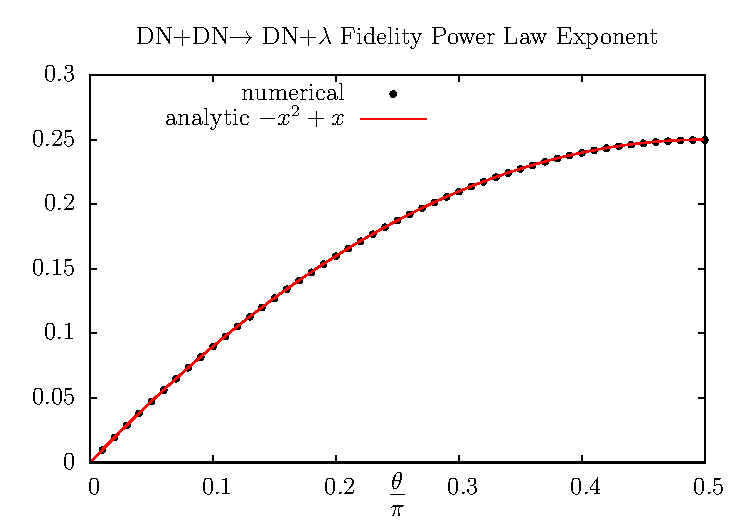
\includegraphics[width=\textwidth]{DN_DN2tan.pdf}
\caption{DN $\rightarrow \lambda$ diagram fidelity power law exponent.}
\end{minipage}
\end{figure}
% flatex input end: [fig_dn_lambda.tex]

\begin{figure}[!h]
% settings for subfigure 1
\begin{minipage}[t]{0.3\linewidth}
\centering
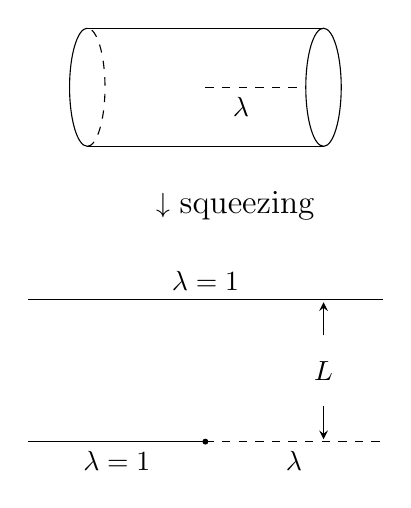
\begin{tikzpicture}[scale = 1.5]
\begin{scope}[shift={(0.5,0)}]
\draw (0,1) arc (90:270:0.15 and 0.5);
\draw[dashed] (0,0) arc (-90:90:0.15 and 0.5);
\draw (0,1) --++(2, 0);
\draw (0,0) --++(2, 0);
\draw[dashed] (1,0.5) --++(0.8, 0);
\node[below] () at (1.3,0.5) {$\lambda$};
\draw (2,0.5) ellipse (0.15 and 0.5);
\end{scope}
\node[right] () at (1,-0.5) {$\downarrow$};
\node[right] () at (1.2,-0.5) {\large squeezing};
\begin{scope}[shift={(0,-2.5)}]
\draw (0,0) -- (1.5,0);
\draw[dashed] (1.5,0) -- (3,0);
\draw[fill] (1.5,0) circle (0.02);
\draw (0,1.2) -- (3,1.2);
\draw[-stealth] (2.5,0.9)--(2.5, 1.18);
\draw[-stealth] (2.5,0.3)--(2.5, 0.02);
\node () at (2.5,0.6) {$L$};
\node[below] () at (0.75,0) {$\lambda = 1$};
\node[below] () at (2.25,0) {$\lambda$};
\node[above] () at (1.5,1.2) {$\lambda = 1$};
\end{scope}
\end{tikzpicture}
\caption{P $\rightarrow \lambda$ diagram before and after squeezing}
\label{fig:P-squeeze}
\end{minipage}
\hfill
% settings for subfigure 2
\begin{minipage}[t]{0.65\linewidth}
\centering
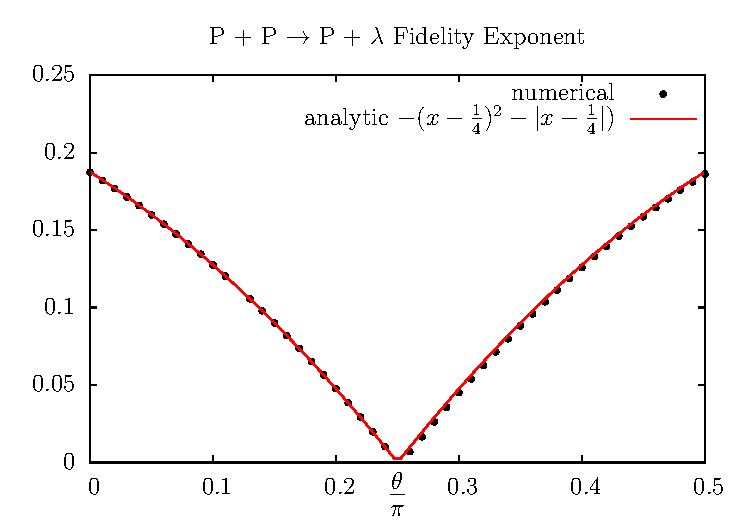
\includegraphics[width=\textwidth]{p_p2tan.pdf}
\caption{DN $\rightarrow \lambda$ diagram fidelity power law exponent.}
\end{minipage}
\end{figure}

Another interesting case is the when the far ends of the initial chains are connected(through periodic or a $\lambda$ interface). The analytic result is
\begin{equation}
\begin{aligned}
  \mathcal{F}( \lambda = 1 \rightarrow \lambda ) &=  \frac{\beta}{2}\Big[  -( x - \frac{1}{4} )^2  + | x - \frac{1}{4} | - \frac{1}{6} \Big]  + {\color{red} \frac{\beta}{12}} \\
  &= \Big[  -( x - \frac{1}{4} )^2  + | x - \frac{1}{4} | \Big]  \ln L \quad x = \frac{\theta}{\pi}, \lambda = \tan \theta 
\end{aligned}
\end{equation}

{\bf A note for the zero mode:} When zero mode is present, the boson groundstate is not well-defined; numerically instability kicks in. Adding a small mass is the common remedy, but doesn't work in the fidelity calculation. What we do here is to perturb the boundary condition by a small angle.

In the DN$\rightarrow \lambda$ diagram, zero mode exists when the two sides of the chain $NN$ boundary condition. The combination DN is actually a $\lambda = 0$ interface. We modify one of them to $\lambda = \tan( 0.001 \pi )$ to avoid the zero mode. In the periodic case, we take the one of them to be $\lambda = \tan(0.251\pi)$ although precise periodic boundary condition corresponds to $\lambda = \tan(\frac{\pi}{4})$. This is a numerical way of regularization that matches with our no-zero-mode analytic calculation. 


%%% Local Variables:
%%% TeX-master: "bCFT_notes"
%%% TeX-PDF-mode: t
%%% End:
% flatex input end: [fidel_num_res.tex]

% configure hyperref to remove ugly boxes from links

\appendix


\section{DN-$\lambda$ Casimir Energy from Groundstate Energy Calculation}
\label{app:gnd_dn_lambda}
% flatex input: [gnd_dn_lambda.tex]


\begin{figure}[h]
\centering
\begin{tikzpicture}[scale = 1]
\draw (0,0)--(0,2);
\draw (1.5,0)--++(0,2);
\node () at (-0.5,1) {DN};
\node () at (1.8,1) {$\lambda$};
\draw[-stealth] (0.75,0.75)--++(0,0.5);
\begin{scope}[shift={(5,0)}]
\draw (0,0)--(0,2);
\draw (3,0)--++(0,2);
\draw[dashed] (1.5,0)--++(0,2);
\node () at (-0.5,1) {N};
\node () at (3.5,1) {D};
\node () at (1.7,1) {$\lambda$};
\end{scope}
\end{tikzpicture}
\caption{Partition function of Hamiltonian with DN and $\lambda$ boundary conditions. The width of the strip is $\pi$ due to folding. We unfold the cylinder and the new stripe have $N$ and $D$ boundary conditions on the left and right plus a $\lambda$ junction in the middle. }
\label{fig:DN-lambda-gnd}
\end{figure}

{\bf Eigenfunction}: 

The unfolded configuration has D/N boundary conditions at $x = \pm \frac{L}{2}$ and linking boundary condition at $x = 0$. The general solutions can be written as
\begin{equation}
f(k, x) = 
\left\lbrace
\begin{aligned}
  A_1 e^{i kt} \cos(kx +\frac{1}{2}kL ) &  \quad x < 0  \\
  A_2 e^{ikt}  \sin(kx - \frac{1}{2}kL ) & \quad x > 0   \\
\end{aligned} \right. 
\end{equation}
At the junction we have $\frac{\partial_x \phi_1}{ \partial_t \phi_1} = \lambda^2 \frac{\partial_x \phi_2}{ \partial_t \phi_2}$, which cancels the $A$s and gives
\begin{equation}
\tan ^2 (\frac{1}{2} kL ) = \lambda^2 
\end{equation}
Hence
\begin{equation}
 \frac{kL}{2} = \pm \theta + n \pi \implies  k = \frac{2\pi}{L}( n \pm \frac{\theta}{\pi} )  \quad \theta \in [0,\frac{\pi}{2} ]  
\end{equation}
The normalized eigenfunctions are
\begin{equation}
f_n(x) = \sqrt{\frac{2}{L}}
\left\lbrace
\begin{aligned}
  \cos(kx +\frac{1}{2}kL ) &  \quad x < 0  \\
  \pm \sin(kx - \frac{1}{2}kL ) & \quad x > 0   \\
\end{aligned} \right. 
\qquad 
k = \frac{2\pi}{L}( n \pm  \frac{\theta}{\pi} )  \quad n \in \mathbb{Z} 
\end{equation}

{\bf Mode Expansion and Casimir Energy}:

Expand the field $\phi = \sum_n \phi_n f_n(x) $, the action and Hamiltonian becomes
\begin{equation}
  S = \frac{g}{2} \int dt \, \sum_{n \in \mathbb{Z} }\left(  \dot{\phi}^2_n + k^2 \phi_n^2 \right) \implies\quad   g \dot{\phi}_n  = \pi_n \quad \implies H =  
\frac{1}{2g}\sum_{n \in \mathbb{Z} } \pi_n^2 + ( kg )^2  \phi_n^2 
\end{equation}
Define the creation and annihilation operators as usual
\begin{equation}
\begin{aligned}
a_n = \frac{1}{\sqrt{2}} ( \sqrt{ |k|g} \phi_n + \frac{i }{\sqrt{|k|g} }\pi_n  ) \\
a^{\dagger}_n = \frac{1}{\sqrt{2}} ( \sqrt{ |k|g} \phi_n - \frac{i }{\sqrt{|k|g} }\pi_n  ) \\
\end{aligned}
\end{equation}
then
\begin{equation}
H = \frac{1}{2} \sum_{n \in \mathbb{Z} } |k|  (a^{\dagger}_n a_n + \frac{1}{2} )
\end{equation}
The Casimir energy is 
\begin{equation}
\begin{aligned}
E_c &= \frac{1}{4} \sum_{n \in \mathbb{Z}} | k| = \frac{\pi}{2L} ( \sum_{n \in \mathbb{Z}}  | n + x | + \sum_{n \in \mathbb{Z}}  | n - x |  )  = \frac{\pi}{L} ( \sum_{n \in \mathbb{Z}}  | n + x |  )\quad x = \frac{\theta}{\pi}\\  
&= \frac{\pi}{L} \Big[\sum_{n \ge 0 } ( n + x )^{-s} + \sum_{n \ge 0 }  ( n - x)^{-s}  +   x^{-s} \Big]\Big|_{s = -1} \\
&= \frac{\pi}{L} \left[ \zeta_{\rm H}( -1, x ) + \zeta_{\rm H}( -1, x ) +  x \right] \\
&= \frac{\pi}{L} ( - x^2 + x - \frac{1}{6})  = \frac{1}{2} ( - x^2 + x - \frac{1}{6})
\end{aligned}
\end{equation}
The free energy is
\begin{equation}
F = \frac{\beta}{2} ( - x^2 + x - \frac{1}{6}) = - \frac{\beta}{2} B_2( x) 
\end{equation}
The full expression also agrees with the boundary state calculation in Eq.~\ref{eq:dn_lambda_bd_state}


%%% Local Variables:
%%% TeX-master: "bCFT_notes"
%%% TeX-PDF-mode: t
%%% End:
% flatex input end: [gnd_dn_lambda.tex]

% configure hyperref to remove ugly boxes from links

\section{$\lambda_1 \rightarrow \lambda_2$ Boundary State Calculation}
\label{app:lambda_12}
% flatex input: [lambda_1_lambda_2.tex]

This calculation is very similar to the presented in App.~\ref{app:casimir_energy_DD_DN}. 

\begin{figure}[h]
\centering
\begin{tikzpicture}[scale = 1]
\draw (0,0)--(2,0);
\draw (0,1.5)--++(2,0);
\node () at (1,-0.5) {$\lambda_1$};
\node () at (1,2) {$\lambda_2$};
\draw[-stealth] (1,0.5)--++(0,0.5);
\end{tikzpicture}
\caption{Partition function between two boundary states $\lambda_1$ and $\lambda_2$}
\label{fig:part-lambda1-lambda2-2}
\end{figure}

The wanted partition function is
\begin{equation}
Z_{ab} = \langle 0 | \exp\Big\{ \vec{b} R_a^* \vec{\bar{b}}\Big\} \exp\Big\{ - \vec{b}^{\dagger} \mathbb{I}_2 \otimes M  \vec{b} \Big\}   \exp\Big\{  \vec{b}^{\dagger} R_b  \vec{\bar{b}}^{\dagger}\Big\}  |0  \rangle  = \frac{1}{\det ( 1 - R^{\dagger} _a  e^{- \mathbb{I}_2 \otimes M} R_b) }
\end{equation}
where
\begin{equation}
M =  \frac{4\pi^2}{\beta} \text{diag}( 1, 2, \cdots )
\end{equation}
$R_a$($R_b$) correspond to the $\lambda_1$ and $\lambda_2$ boundary conditions. Using the fact that their determinants are $\det( R_a R_b^{\dagger})  = 1$, we have
\begin{equation}
\begin{aligned}
F &= - \ln Z_{ab} = \ln \det( 1 - R^{\dagger} _a  e^{- \mathbb{I}_2 \otimes M} R_b ) = \ln \det ( R_a R_b^{\dagger} - e^{- \mathbb{I}_2 \otimes M} )\\
& = \ln \det 
\begin{bmatrix}
\cos 2 \Delta \theta \mathbb{I} - e^{-M}   & \sin 2 \Delta \theta \mathbb{I}\\
- \sin 2\Delta \theta \mathbb{I}  &   \cos 2 \Delta \theta \mathbb{I} - e^{-M} \\ 
\end{bmatrix} \quad \text{where } \Delta \theta = \theta_2 - \theta_1 \\
& = \sum_i \ln [ 1 - 2 \cos 2 \Delta \theta e^{- \lambda_i } + e^{- 2 \lambda_i }  ] \\
& = \frac{\beta}{4\pi^2} \int_0^{\infty} dx \ln [ 1 - 2 \cos 2 \Delta \theta e^{-x} + e^{-2x} ] 
\end{aligned}
\end{equation}
This integral is an even function of $\Delta \theta$ and the $\Delta \theta > 0$ case reduce to the polylog and Bernoulli polynomial
\begin{equation}
\begin{aligned}
  F &= \frac{\beta}{4\pi^2} \left[ - \text{Li}_2 ( e^{2i |\Delta \theta|} ) - \text{Li}_2 ( e^{- 2i |\Delta \theta|} ) \right]  = \frac{\beta}{4\pi^2}  \left[ - 2\pi^2 B_2 (x) \right] \\
  &= - \frac{\beta}{2} B_2( |x| ) = \frac{\beta}{2} (|x| - x^2 - \frac{1}{6}) \quad x = \frac{\Delta \theta}{ \pi} \\
\end{aligned}
\end{equation}

%%% Local Variables:
%%% TeX-master: "bCFT_notes"
%%% TeX-PDF-mode: t
%%% End:
% flatex input end: [lambda_1_lambda_2.tex]

% configure hyperref to remove ugly boxes from links

\section{Determinant Identity for Amplitude between Boundary States}
\label{app:pf_of_id}
% flatex input: [pf_of_id.tex]

For real symmetric matrix $M$
\begin{equation}
\exp\Big\{- \vec{b}^{\dagger} M \vec{b}  \Big\} \exp \Big\{ \vec{b}^{\dagger} R \bar{\vec{b}}^{\dagger}  \Big\}  = \exp \Big\{ \vec{b}^{\dagger} e^{-M}  R \bar{\vec{b}}^{\dagger}  \Big\} \exp\Big\{- \vec{b}^{\dagger} M \vec{b}  \Big\} 
\end{equation}

{\bf Proof:}  
We first restrict to the case when $R = I$. To avoid confusion, we assume the daggered vector are row vectors and write $\exp \Big\{ \vec{b}^{\dagger} R \bar{\vec{b}}^{\dagger}  \Big\} $ as $\exp \Big\{ \vec{b}^{\dagger} R \bar{\vec{b}}^{*}  \Big\} $. 

{\it Diagonal Basis}: We diagonalize $M = O^{T} \Lambda O $ and rotate the two sets of boson operators to the diagonal basis
\begin{equation}
  \vec{b}^{\dagger}  M \vec{b} = \vec{d}^{\dagger} \Lambda \vec{d}  \quad \vec{d} = O \vec{b} \quad \vec{\bar{d}}^{*} = O^T \vec{\bar{b}}^{*}
\end{equation}
so that the whole expression can be written as
\begin{equation}
\begin{aligned}
  \exp&\Big\{- \vec{b}^{\dagger} M \vec{b}  \Big\} \exp \Big\{ \vec{b}^{\dagger} \bar{\vec{b}}^{*}  \Big\}  =  
  \exp\Big\{- \vec{d}^{\dagger} \Lambda \vec{d}  \Big\} \exp \Big\{   \vec{d}^{\dagger} \bar{\vec{d}}^{*}  \Big\} \\
& = \prod_i  \exp\Big\{- \lambda_i d_i^{\dagger} d_i  \Big\} \exp \Big\{  d_i^{\dagger} \bar{d}_i ^{\dagger}  \Big\}
\end{aligned}
\end{equation}
{\it Baker-Campbell-Hausdorff formula}: For $ [X, Y] = sY $, we have a solvable case of Baker-Campbell-Hausdorff formula
\begin{equation}
  e^X e^{Y} = e^{\exp (s ) Y} e^{X}
\end{equation}
Taking $X = -\lambda_i d_i^{\dagger} d_i$, $Y = d_i^{\dagger}, \bar{d}^{\dagger}$, we have
\begin{equation}
[- \lambda_i d_i^{\dagger} d_i, d_i ^{\dagger} \bar{d}_i^{\dagger}] =  - \lambda_i  d_i ^{\dagger} \bar{d}_i^{\dagger} 
\end{equation}
and so $s = - \lambda_i$ for each $\lambda_i$. This enable us to commute those exponentials
\begin{equation}
\begin{aligned}
 \exp\Big\{- \vec{b}^{\dagger} M \vec{b}  \Big\} \exp \Big\{  \vec{b}^{\dagger} \bar{\vec{b}}^{*}  \Big\}   &= \prod_i \exp \Big\{ \alpha e^{- \lambda_i }  d^{\dagger}_i \bar{d}^{\dagger}_i  \Big\}  \exp \Big\{-\lambda_i  d^{\dagger}_i d_i  \Big\} \\
 & = \exp \Big\{ \vec{b}^{\dagger} e^{-M}  \bar{\vec{b}}^{*}  \Big\} \exp\Big\{- \vec{b}^{\dagger} M \vec{b}  \Big\} 
\end{aligned}
\end{equation}

{\it The General Case}: When $R \ne I$, we take $\vec{\bar{d}}^* = O^T R \vec{\bar{b}}^*$. The role of $\bar{b}$ is decorative; it is effectively a $c$-number and we only use its independence w.r.t. $\vec{b}$. Hence the rest of the proof follows the same way. 

{\bf Corollary :} 
\begin{equation}
Z_{ab} = \langle 0 | \exp\Big\{ \vec{b} R_a^* \vec{\bar{b}}\Big\} \exp\Big\{ - \vec{b}^{\dagger} M  \vec{b} \Big\}   \exp\Big\{  \vec{b}^{\dagger} R_b  \vec{\bar{b}}^{\dagger}\Big\}  |0  \rangle  = \frac{1}{\det( 1- R_a^{\dagger} e^{-M} R_b )} 
\end{equation}
{\bf Proof:}

Using the identity we have just proved, 
\begin{equation}
Z_{ab} =   \langle 0 | \exp\Big\{ \vec{b} R_a^* \vec{\bar{b}}\Big\}  \exp \Big\{ \vec{b}^{\dagger} e^{-M}  R_b \bar{\vec{b}}^{\dagger}  \Big\}  |0 \rangle 
\end{equation}
A direct application of the MacMahon master theorem
\begin{equation}
  \langle 0 | \exp \Big\{ \vec{b}_1 X \vec{b}_2 \Big\}  \exp \Big\{ \vec{b}^{\dagger}_1 Y \vec{b}^{\dagger}_2 \Big\}|0  \rangle 
 = \frac{1}{\det(1 - X^T Y )}
\end{equation}
proves the result. 


%%% Local Variables:
%%% TeX-master: "bCFT_notes"
%%% TeX-PDF-mode: t
%%% End:
% flatex input end: [pf_of_id.tex]


\bibliographystyle{unsrt}
\bibliography{bCFT_notes}

\end{document}
%%% Local Variables: 
%%% TeX-PDF-mode: t
%%% End:
% flatex input end: [bCFT_notes.tex]
